\documentclass{beamer}
% Try the class options [notes], [notes=only], [trans], [handout],
% [red], [compress], [draft] and see what happens!

% \usepackage{definitions}
\usepackage[british]{babel}
\usepackage{color, soul}

%% tikz tricks
% \tikzset{onslide/.code args={<#1>#2}{%
%   \only<#1>{\pgfkeysalso{#2}} 
% }}

\pdfinfo{
        /Title (cim)
        /Creator (LaTeX)
        /Producer (pdflatex)
        /Author (szerzo)
        /CreationDate (datum)
	/Subject (tema)
}


\mode<article> % only for the article version
{
  \usepackage{fullpage}
  \usepackage{hyperref}
}
\mode<presentation>
{
  \usetheme[left,width=0.65in,height=0.55in]{Kolozsvar}
  \setbeamercovered{transparent}
  \setbeamertemplate{navigation symbols}{}
  \setbeamertemplate{footline}%
     {\vspace*{-1.4em}\hspace*{0.66in}\textbf{\insertframenumber/\inserttotalframenumber}\newline\vspace*{0.4em}}
		\setbeamerfont{block title}{size=\larger} % RELSIZE -- html-sizes 
		\usefonttheme{professionalfonts}
		\setbeamercolor{math text}{fg=green!30!red!30!brown}
		\setbeamercolor{normal text in math text}{parent=math text}
}

\setbeamercovered{dynamic}

% The following info should normally be given in you main file:
\title[Apache Kafka]{Apache Kafka}
%
\author{ Hunor Ördög, Norbert-Raymond Pap}
%
\institute[UBB Cluj-Napoca]{
  Department of Mathematics and Informatics\\
  Babe{\c{s}}--Bolyai University, Cluj-Napoca}
%
\date{2024 May}


\begin{document}

\frame{\maketitle}

\mode<presentation>
{
  % \begin{frame}
  %   \frametitle{Talk structure}
  % \tableofcontents
  % \end{frame} 

  % \AtBeginSection[]
  {
      \begin{frame}<beamer>{Contents}
        % \tableofcontents[currentsection,currentsubsection,hideothersubsections]
        \tableofcontents
      \end{frame}
    }
}

%%%%%%%%%%%%%%%%%%%%%%%%%%%%%%%%%%%%%%%%%%%%%%%%%%%%%%%%%%%%%%%%%%%%%%
\section[What is Kafka?]{What is Kafka?}

\begin{frame}{What is Kafka?}
  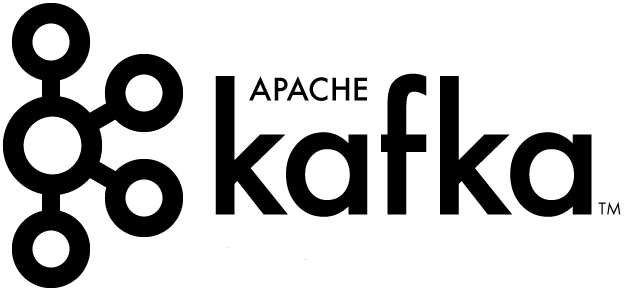
\includegraphics[scale=0.25]{fig/kafka_logo.png}
  \vspace*{2em}
  \begin{itemize}
    \item Open-source \underline{distributed event streaming platform}.
  \end{itemize}
\end{frame}

\begin{frame}{What is a “distributed streaming platform”?}
  \begin{itemize}
    \item Streams are just infinite data, data that never ends.
    \item Distributed means Kafka works in a cluster, each node in the cluster is called a \textbf{Broker}.
          % Brokers are just servers executing a copy of apache kafka.
          \vspace*{1em}
    \item Kafka is a set of machines working together to be able to handle and process real-time infinite data.
  \end{itemize}
\end{frame}


\begin{frame}{Where does Kafka come from?}
  \begin{itemize}
    \item Kafka was originally developed at LinkedIn 
\includegraphics[scale=0.006]{fig/linkedin_logo.png} in 2010
    \item Open sourced in early 2011
  \end{itemize}
  
\includegraphics[scale=0.17]{fig/apache_software.png}
\end{frame}
% 2012 ota Apache Kafka neven ismert es azota ok tartsak karban

\section[Kafka components \& Internal Architecture]{Kafka components \& Internal Architecture}

\begin{frame}{Kafka Components}
  \begin{itemize}
    \item \hl{Producer}
    \item Consumer
    \item Broker
    \item Topic
    \item Partitions
    \item Offset
    \item Consumer Groups
    \item Zookeeper
  \end{itemize}
\end{frame}

\begin{frame}{Kafka Components}{Producer}

\end{frame}

\begin{frame}{Kafka Components}
  \begin{itemize}
    \item Producer
    \item \hl{Consumer}
    \item Broker
    \item Topic
    \item Partitions
    \item Offset
    \item Consumer Groups
    \item Zookeeper
  \end{itemize}
\end{frame}

\begin{frame}{Kafka Components}{Consumer}

\end{frame}

\begin{frame}{Kafka Components}
  \begin{itemize}
    \item Producer
    \item Consumer
    \item \hl{Broker}
    \item Topic
    \item Partitions
    \item Offset
    \item Consumer Groups
    \item Zookeeper
  \end{itemize}
\end{frame}

\begin{frame}{Kafka Components}{Broker}

\end{frame}

\begin{frame}{Kafka Components}
  \begin{itemize}
    \item Producer
    \item Consumer
    \item Broker
    \item \hl{Topic}
    \item Partitions
    \item Offset
    \item Consumer Groups
    \item Zookeeper
  \end{itemize}
\end{frame}

\begin{frame}{Kafka Components}{Topic}

\end{frame}

\begin{frame}{Kafka Components}
  \begin{itemize}
    \item Producer
    \item Consumer
    \item Broker
    \item Topic
    \item \hl{Partitions}
    \item Offset
    \item Consumer Groups
    \item Zookeeper
  \end{itemize}
\end{frame}

\begin{frame}{Kafka Components}{Partitions}

\end{frame}

\begin{frame}{Kafka Components}
  \begin{itemize}
    \item Producer
    \item Consumer
    \item Broker
    \item Topic
    \item Partitions
    \item \hl{Offset}
    \item Consumer Groups
    \item Zookeeper
  \end{itemize}
\end{frame}

\begin{frame}{Kafka Components}{Offset}

\end{frame}

\begin{frame}{Kafka Components}
  \begin{itemize}
    \item Producer
    \item Consumer
    \item Broker
    \item Topic
    \item Partitions
    \item Offset
    \item \hl{Consumer Groups}
    \item Zookeeper
  \end{itemize}
\end{frame}

\begin{frame}{Kafka Components}{Consumer Groups}

\end{frame}

\begin{frame}{Kafka Components}
  \begin{itemize}
    \item Producer
    \item Consumer
    \item Broker
    \item Topic
    \item Partitions
    \item Offset
    \item Consumer Groups
    \item \hl{Zookeeper}
  \end{itemize}
\end{frame}

\begin{frame}{Kafka Components}{Zookeeper}

\end{frame}

\end{document}
